\section{Corba\-Consumer Class Reference}
\label{classCorbaConsumer}\index{CorbaConsumer@{CorbaConsumer}}
Inheritance diagram for Corba\-Consumer::\begin{figure}[H]
\begin{center}
\leavevmode
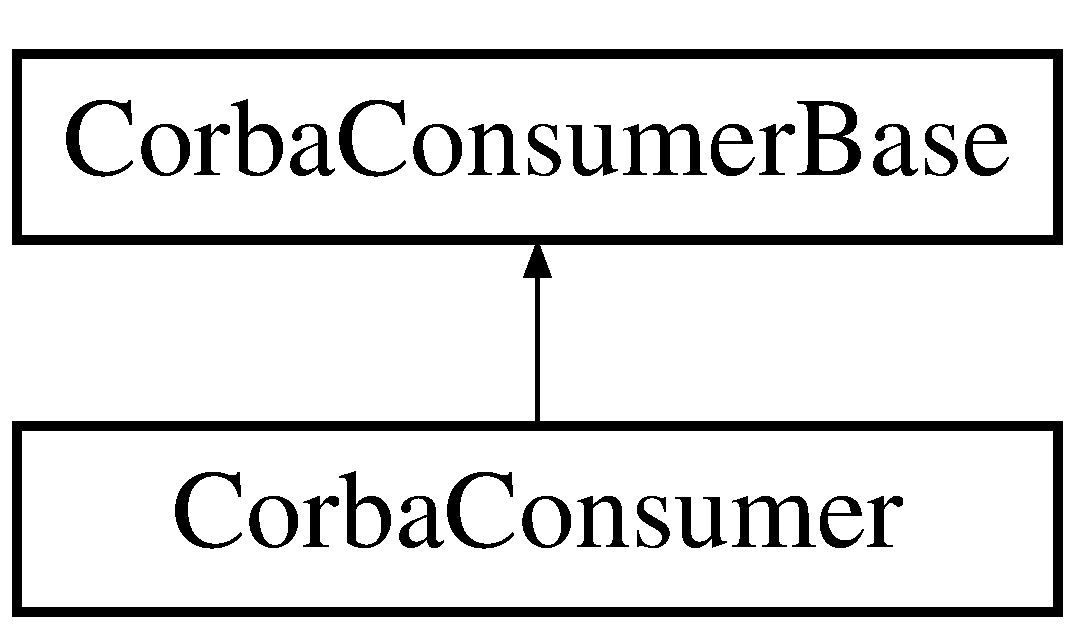
\includegraphics[height=2cm]{classCorbaConsumer}
\end{center}
\end{figure}
\subsection*{Public Member Functions}
\begin{CompactItemize}
\item 
{\bf \_\-\_\-init\_\-\_\-} (interface\-Type=None, consumer=None)
\begin{CompactList}\small\item\em Consructor. \item\end{CompactList}\item 
{\bf equal} (consumer)
\item 
{\bf \_\-\_\-del\_\-\_\-} ()
\begin{CompactList}\small\item\em Destructor. \item\end{CompactList}\item 
{\bf set\-Object} (obj)
\begin{CompactList}\small\item\em Set Object Override function of Consumer\-Base. This operation set an Object to self.\_\-objref in the {\bf Corba\-Consumer\-Base}{\rm (p.\,\pageref{classCorbaConsumerBase})} class, and this object is narrowed to given interface\-Type parameter and stored in the member variable. \item\end{CompactList}\item 
{\bf \_\-ptr} ()
\begin{CompactList}\small\item\em Get Object reference narrowed as interface\-Type. \item\end{CompactList}\item 
{\bf release\-Object} ()
\item 
{\bf \_\-\_\-init\_\-\_\-} (consumer=None)
\begin{CompactList}\small\item\em Consructor. \item\end{CompactList}\item 
{\bf get\-Object} ()
\begin{CompactList}\small\item\em Set CORBA Object. \item\end{CompactList}\end{CompactItemize}


\subsection{Member Function Documentation}
\index{CorbaConsumer@{Corba\-Consumer}!__del__@{\_\-\_\-del\_\-\_\-}}
\index{__del__@{\_\-\_\-del\_\-\_\-}!CorbaConsumer@{Corba\-Consumer}}
\subsubsection{\setlength{\rightskip}{0pt plus 5cm}Corba\-Consumer::\_\-\_\-del\_\-\_\- ()}\label{classCorbaConsumer_CorbaConsumera2}


Destructor. 



Reimplemented from {\bf Corba\-Consumer\-Base} {\rm (p.\,\pageref{classCorbaConsumerBase_CorbaConsumerBasea2})}.\index{CorbaConsumer@{Corba\-Consumer}!__init__@{\_\-\_\-init\_\-\_\-}}
\index{__init__@{\_\-\_\-init\_\-\_\-}!CorbaConsumer@{Corba\-Consumer}}
\subsubsection{\setlength{\rightskip}{0pt plus 5cm}Corba\-Consumer\-Base::\_\-\_\-init\_\-\_\- (consumer = {\tt None})\hspace{0.3cm}{\tt  [inherited]}}\label{classCorbaConsumerBase_CorbaConsumerBasea0}


Consructor. 

\index{CorbaConsumer@{Corba\-Consumer}!__init__@{\_\-\_\-init\_\-\_\-}}
\index{__init__@{\_\-\_\-init\_\-\_\-}!CorbaConsumer@{Corba\-Consumer}}
\subsubsection{\setlength{\rightskip}{0pt plus 5cm}Corba\-Consumer::\_\-\_\-init\_\-\_\- (interface\-Type = {\tt None}, consumer = {\tt None})}\label{classCorbaConsumer_CorbaConsumera0}


Consructor. 

\index{CorbaConsumer@{Corba\-Consumer}!_ptr@{\_\-ptr}}
\index{_ptr@{\_\-ptr}!CorbaConsumer@{Corba\-Consumer}}
\subsubsection{\setlength{\rightskip}{0pt plus 5cm}Corba\-Consumer::\_\-ptr ()}\label{classCorbaConsumer_CorbaConsumera4}


Get Object reference narrowed as interface\-Type. 

This operation returns object reference narrowed as interface\-Type. To use the returned object reference, reference have to be set by {\bf set\-Object()}{\rm (p.\,\pageref{classCorbaConsumer_CorbaConsumera3})}. If object is not set, this operation returns nil object reference. \begin{Desc}
\item[Returns:]The object reference narrowed as interface\-Type\end{Desc}
\index{CorbaConsumer@{Corba\-Consumer}!equal@{equal}}
\index{equal@{equal}!CorbaConsumer@{Corba\-Consumer}}
\subsubsection{\setlength{\rightskip}{0pt plus 5cm}Corba\-Consumer::equal (consumer)}\label{classCorbaConsumer_CorbaConsumera1}




Reimplemented from {\bf Corba\-Consumer\-Base} {\rm (p.\,\pageref{classCorbaConsumerBase_CorbaConsumerBasea1})}.\index{CorbaConsumer@{Corba\-Consumer}!getObject@{getObject}}
\index{getObject@{getObject}!CorbaConsumer@{Corba\-Consumer}}
\subsubsection{\setlength{\rightskip}{0pt plus 5cm}Corba\-Consumer\-Base::get\-Object ()\hspace{0.3cm}{\tt  [inherited]}}\label{classCorbaConsumerBase_CorbaConsumerBasea4}


Set CORBA Object. 

return The CORBA Object reference that given by {\bf set\-Object(obj)}{\rm (p.\,\pageref{classCorbaConsumerBase_CorbaConsumerBasea3})} \begin{Desc}
\item[Returns:]obj Object reference of CORBA object\end{Desc}
\index{CorbaConsumer@{Corba\-Consumer}!releaseObject@{releaseObject}}
\index{releaseObject@{releaseObject}!CorbaConsumer@{Corba\-Consumer}}
\subsubsection{\setlength{\rightskip}{0pt plus 5cm}Corba\-Consumer::release\-Object ()}\label{classCorbaConsumer_CorbaConsumera5}




Reimplemented from {\bf Corba\-Consumer\-Base} {\rm (p.\,\pageref{classCorbaConsumerBase_CorbaConsumerBasea5})}.\index{CorbaConsumer@{Corba\-Consumer}!setObject@{setObject}}
\index{setObject@{setObject}!CorbaConsumer@{Corba\-Consumer}}
\subsubsection{\setlength{\rightskip}{0pt plus 5cm}Corba\-Consumer::set\-Object (obj)}\label{classCorbaConsumer_CorbaConsumera3}


Set Object Override function of Consumer\-Base. This operation set an Object to self.\_\-objref in the {\bf Corba\-Consumer\-Base}{\rm (p.\,\pageref{classCorbaConsumerBase})} class, and this object is narrowed to given interface\-Type parameter and stored in the member variable. 



Reimplemented from {\bf Corba\-Consumer\-Base} {\rm (p.\,\pageref{classCorbaConsumerBase_CorbaConsumerBasea3})}.

The documentation for this class was generated from the following file:\begin{CompactItemize}
\item 
{\bf Corba\-Consumer.py}\end{CompactItemize}
